\tikzstyle{decision} = [diamond, draw, fill=blue!20,
    text width=6em, text badly centered, inner sep=0pt]
\tikzstyle{block} = [rectangle, draw=Mat, fill=blue!20,
    text width=7em, text centered, rounded corners, minimum height=6em]
%\tikzstyle{line} = [draw, ultra thick, color=black!50, -latex']
\tikzstyle{line} = [draw=black,solid,line width=2mm,fill=black,
preaction={-triangle 90,ultra thick,draw,shorten >=-1mm}]
\tikzstyle{cloud} = [draw, ellipse,fill=red!20, 
    minimum height=2em]
%\tikzstyle{noArrow} = [draw, ultra thick, color=black!50]
\tikzstyle{noArrow} = [draw=black,solid,line width=2mm,fill=black]

\begin{tikzpicture}[node distance = 12cm]
	% Nodes
	\node (eeg) {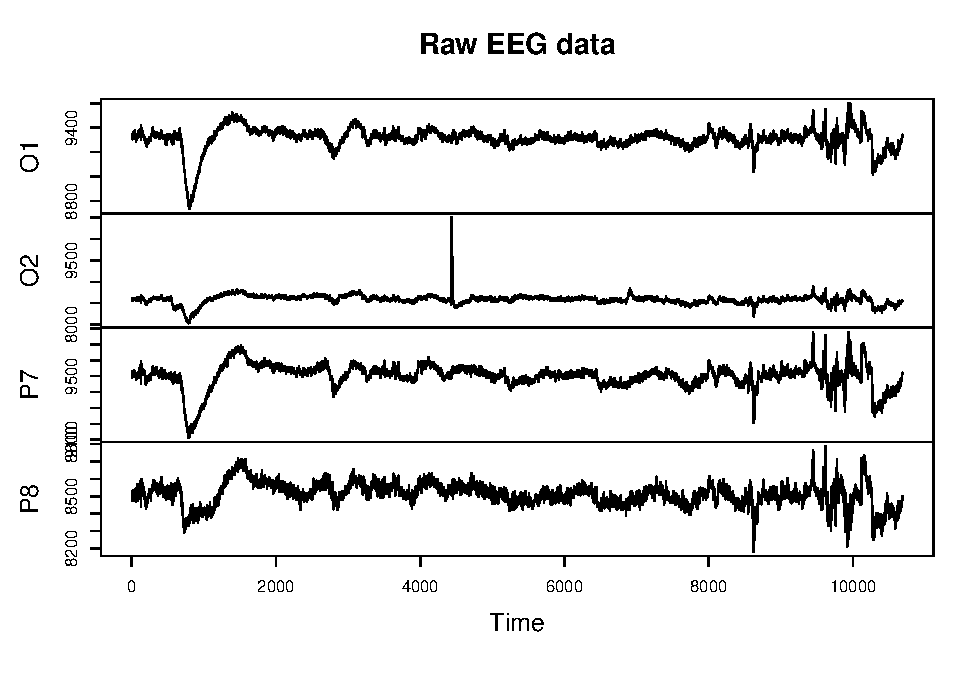
\includegraphics[width=30cm]{./img/eeg.pdf}};
	\coordinate [right of=eeg, node distance=39cm] (dummy2);
	\node [below of=dummy2, node distance=3cm, align=center] (dots) {$\bullet$\\$\bullet$\\$\bullet$};
	\coordinate [left of=dots, node distance=15.5cm] (dummy);
	\coordinate [left of=dummy2, node distance=15.5cm] (dummy3);
	\node [above of=dots] (cca) {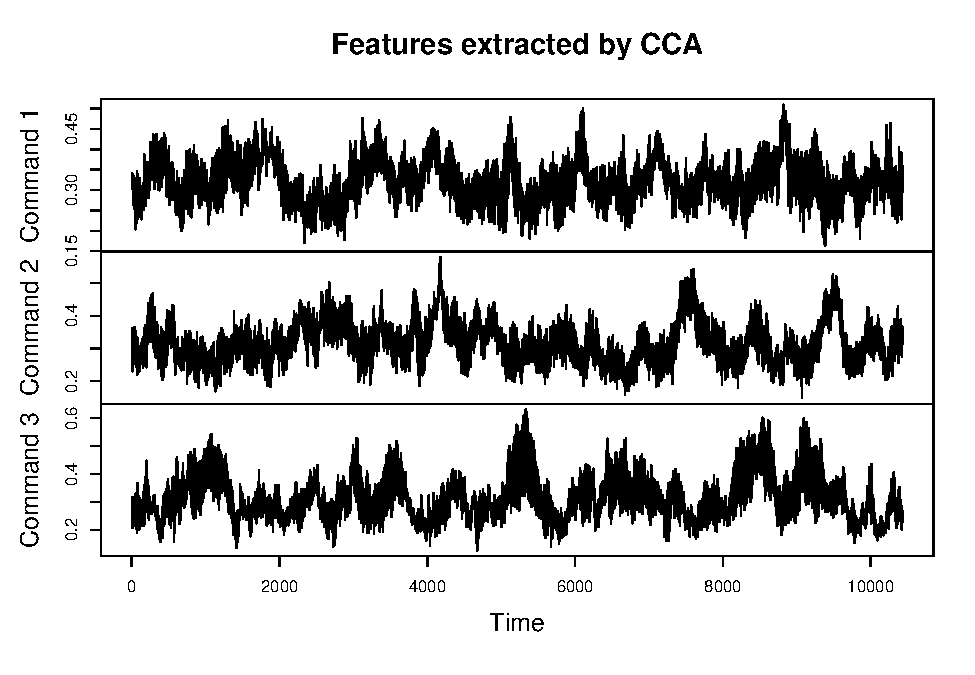
\includegraphics[width=30cm]{./img/cca_features.pdf}};
	\node [below of=dots] (psda) {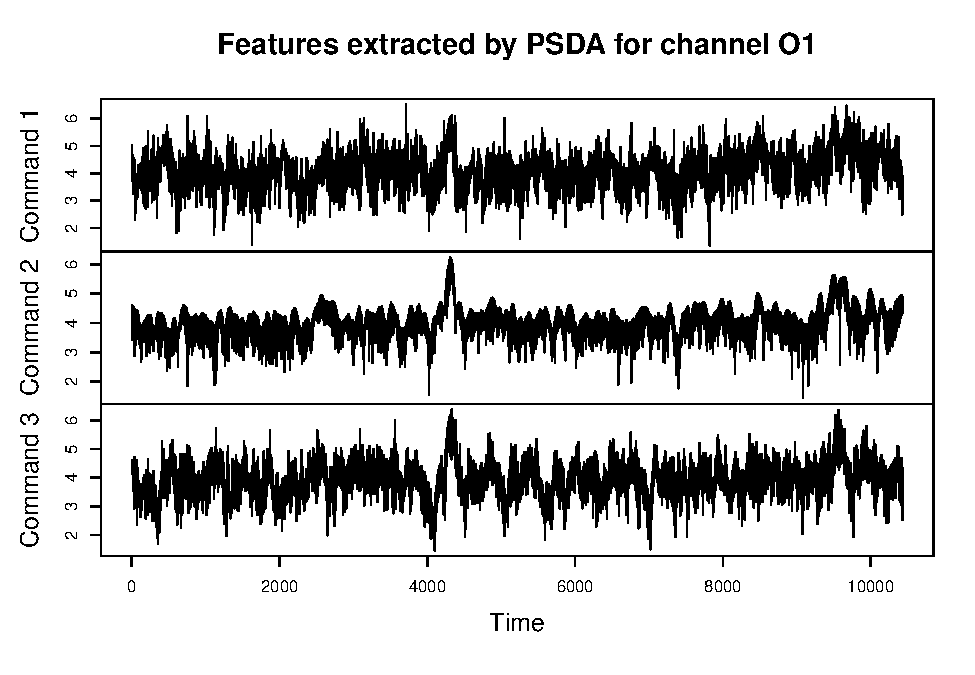
\includegraphics[width=30cm]{./img/psda_features.pdf}};

	\path [line] (eeg) -- (cca);
	\path [line] (eeg) -- (dummy);
	\path [line] (eeg) -- (dummy3);
	\path [line] (eeg) -- (psda);
	
%	% Arrows
%	\path [noArrow] (identification) -- (dummyRight);
%	\path [noArrow] (dummyRight) -- node [color=black, pos=0.5, above] {\textbf{visual feedback}} (dummyLeft);
%	\path [line] (dummyLeft) -- (monitor);
%	\path [line] (identification) -- node [color=black, above] {\textbf{command}} (robot);
%	\path [line] (extraction) -- (identification);
%	\path [line] (processing) -- (extraction);
%	\path [line] (emotiv) -- (processing);
%	\path [line] (brain) -- (emotiv);
	


\end{tikzpicture}
